
\documentclass[letterpaper]{article}
\usepackage{dcj}
\usepackage{lscape}
\usepackage{comment}
\usepackage{geometry}
\usepackage{graphicx}
\usepackage{fontspec}

\geometry{left=1.5in,right=1.5in, top=1in, bottom=1in}

\title{SUPPLEMENTARY:\\Correcting for bias in high-throughput sequencing data}
\author{Daniel C. Jones}


\begin{document}


\dcjtitle{\sc{(SUPPLEMENTARY)}}{\sc{Correcting for Bias in High-Throughput
Sequencing Data}}{Daniel C. Jones}


\section{Trimming Reads}

Observing the nonuniform distribution of nucleotide frequencies surrounding the
5' end of reads, a natural step to take would be to trim the 5' end before mapping,
in the hope that simply removing the portion of the read in which the bias
occurs will also remove the bias. The figure below demonstrates that this is not
the case. Trimming the initial heptamer in the Mortazavi data set does nothing to
reduce the bias, and simply shifts the plot by seven positions. This indicates
that the issue is \emph{sampling bias}, rather than a bias in base calling.


\begin{center}
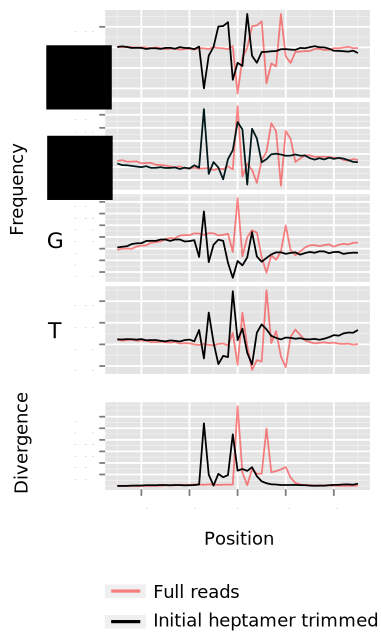
\includegraphics[width=0.35\textwidth]{fig/trimmed-freqs.pdf}
\end{center}



\section{Additional Kullback-Leibler Divergence Plots}

Below we plot the adjusted and unadjusted KL divergence plots, supplementing
those in the results section of the main paper.


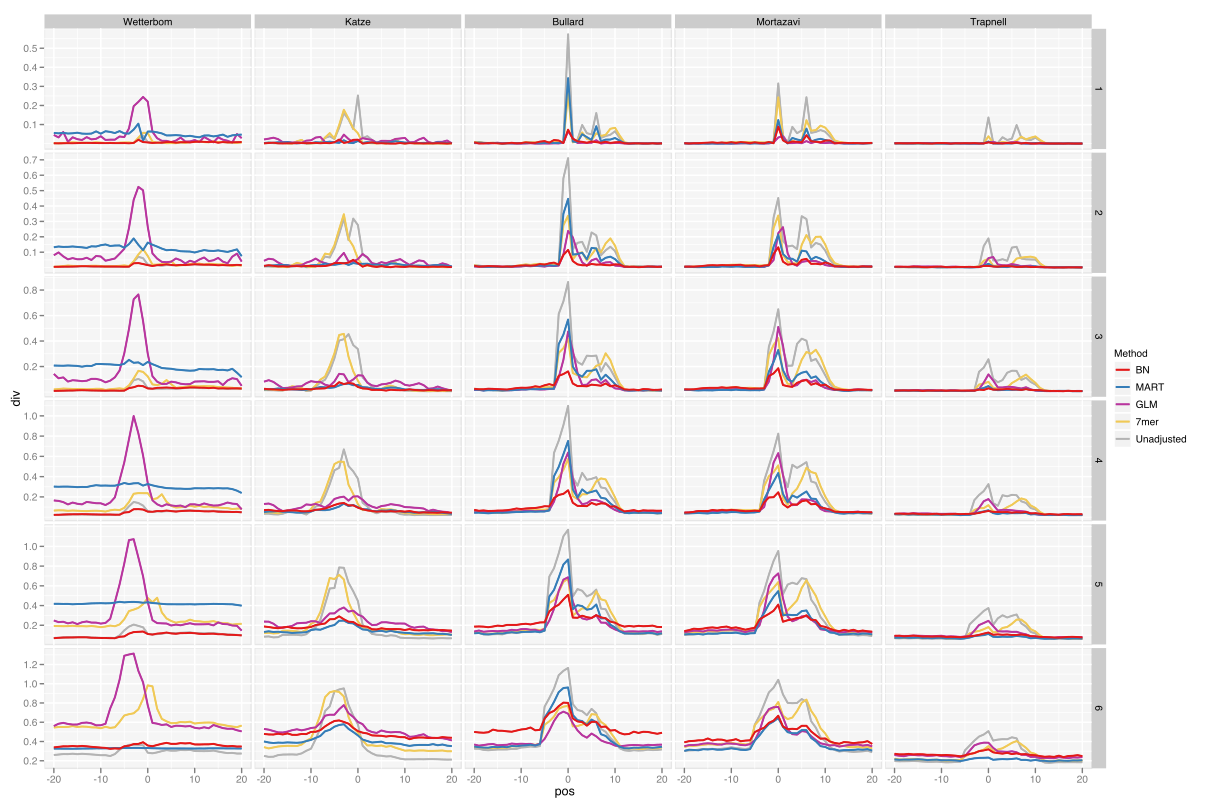
\includegraphics[width=\textwidth]{fig/kl-all.pdf}




\section{Runtime-Accuracy Trade-off}

Training our model on more reads results in more accurate estimation of bias,
but a longer training time. Here we investigate that trade-off by training our
model on progressively more reads from the Mortazavi data set. We use the
median pseudo-coefficient of determination ($R^2$) over exons selected for our
test set. Each point is additionally labeled with the time used to train the
model on one core of a 3Ghz Intel Xeon processor.

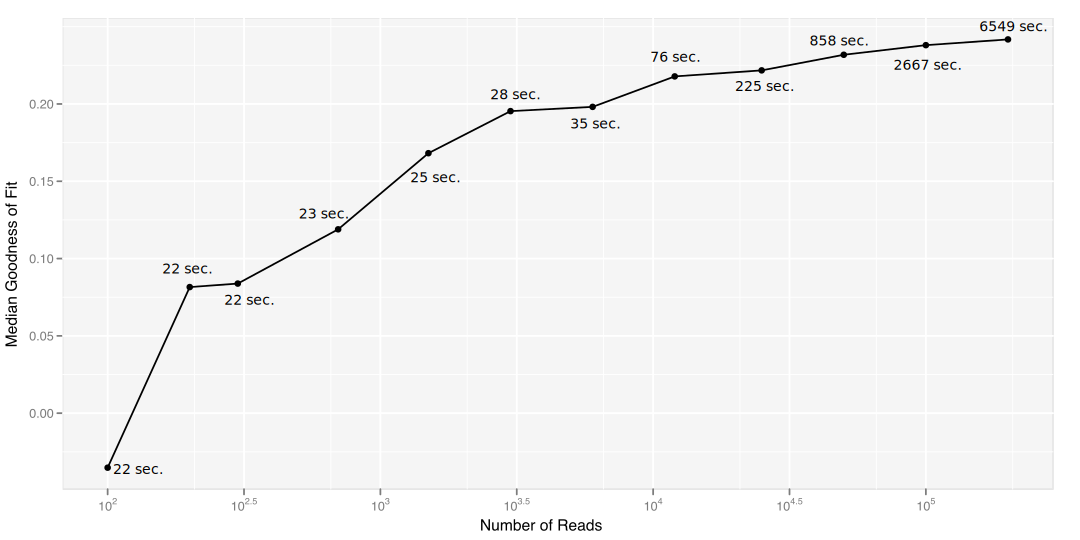
\includegraphics[width=\textwidth]{fig/pois-n.eps}


\section{Sensitivity of Parameters}

The performance of our method is dependent on two parameters: the standard
deviation at which background sequences are sampled, and the degree to which
model complexity in penalized. We have also introduced parameters limiting the
number of parents a node may have ($p_{\text{max}}$) as well as the distance
that an edge may traverse ($d_{\text{max}}$), but these exist only to control
the amount of CPU time used and have a much simpler interpretation: bigger is
better, but slower.

Here we retrain the model on 50,000 reads from the Mortazavi data
set, varying these first two parameters to assess the sensitivity of the
observed results to their values.

\begin{center}
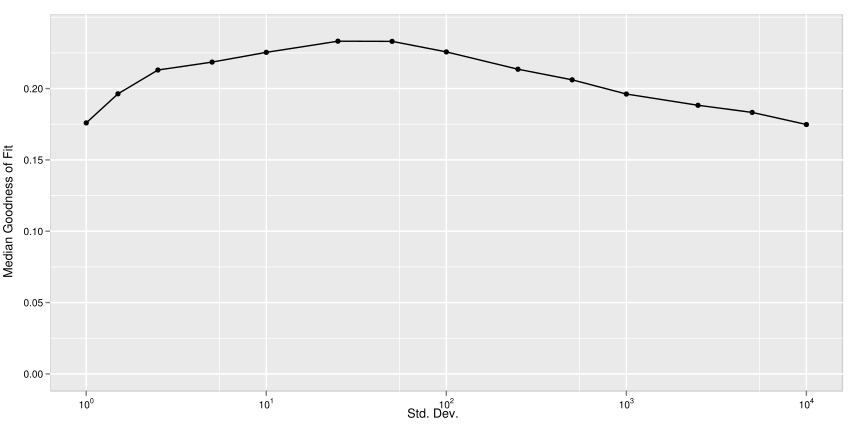
\includegraphics[width=0.8\textwidth]{fig/pois-sampstd.pdf}
\end{center}

The above plot show the standard deviation used to draw background samples
varied from 1 to 10,000. Apparent from this plot is that, while the optimal
choice lies somewhere between 10 and 100, the model performs competitively for
any reasonable value.


\begin{center}
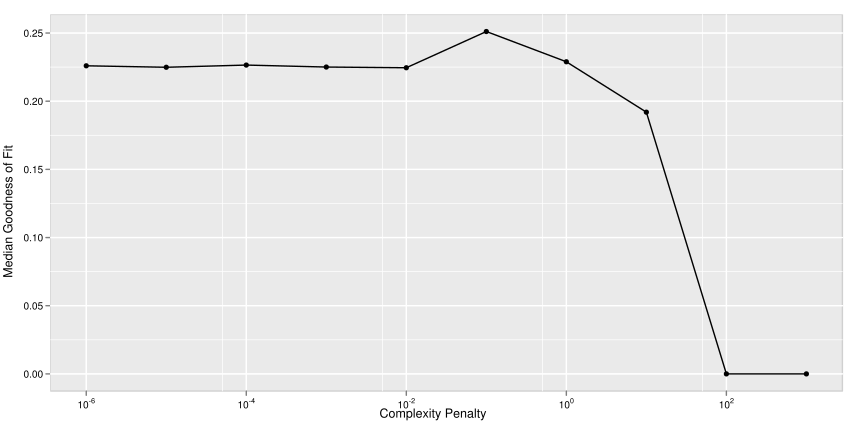
\includegraphics[width=0.8\textwidth]{fig/pois-comppen.pdf}
\end{center}

Here we multiply the complexity penalty term of the BIC by constants varying
from $10^{-6}$ to $10^{3}$. (Recall that the BIC is $2\ell - m \log n$ where
$\ell$ is the log-likelihood, $m$ is the number of parameters needed to specify
the model, and $n$ is the number of training examples. Here we compute $2 \ell -
c m \log n$, varying $c$.)

It is clear from the above figure, that a very severe complexity penalty will
result in a poor model. Here, for constants larger than 100, an empty model is
trained, resulting in the goodness of fit of 0. Conversely, if this constant is
very small, a overly-dense model will be trained.  In this data, for constants
less than 0.01, the maximally dense model is trained (given the restraints on
in-degree and edge distance). This result is a sub-optimal but entirely adequate
solution.


\section{ChIP-Seq}

Though the MART model \cite{Li2010} performed very well in several cases, ours
offers the advantage that no gene annotations are required for training.  In
RNA-Seq this is useful in applications of de-novo gene discovery, but it also
allows our method to be applied to ChIP-Seq and other short read data. Here we
examine one publicly available ChIP-Seq data set from Cao, et. al.
\cite{Cao2010}. Specifically, we used one run, with Sequence Read Archive
accession number SRR034831, containing 3,873,192 reads. These were mapped to the
reference genome using Bowtie \cite{Langmead2009}, resulting in 1,382,867
uniquely mapped reads, which were used for this analysis.

Measuring nucleotide frequencies, we find the bias to be significantly less
than that observed the RNA-Seq data sets we tested, but the data was by no means
unbiased.

\begin{center}
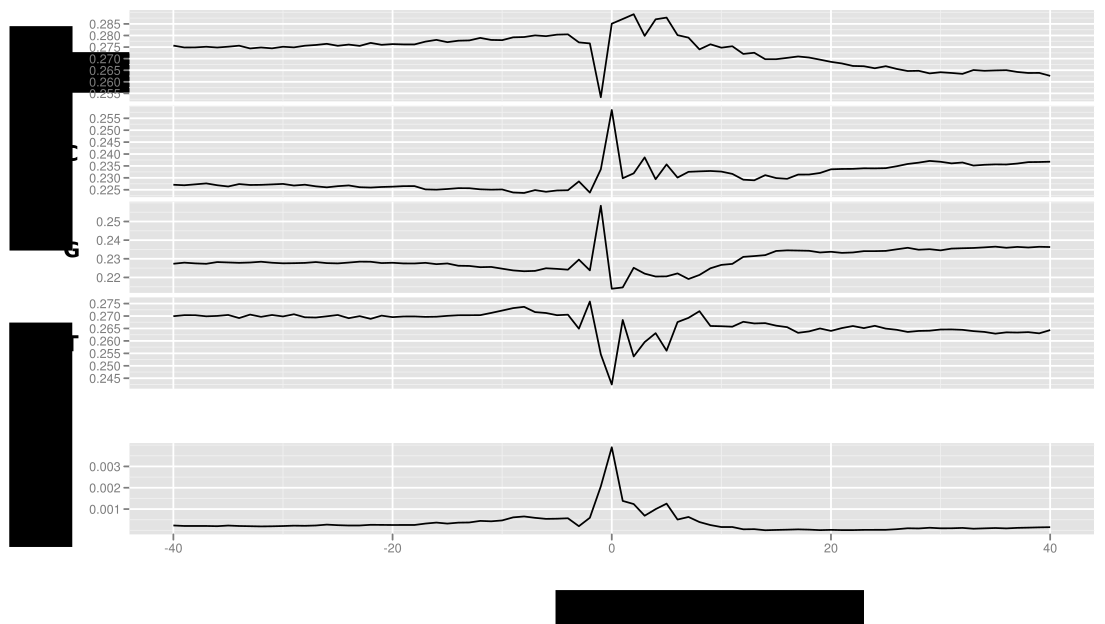
\includegraphics[width=0.7\textwidth]{fig/freqs_cao.pdf}
\end{center}

In the analysis of the RNA-Seq data, we used the assumption of continuous
transcription across annotated exons to evaluate the efficacy of the models, as
well as to train the GLM and MART models. Evaluating bias correction on ChIP-Seq
data necessitates dropping the Poisson regression test, as well as the GLM and
MART models from our comparison, which can not be applied to such data.

We did however repeat our analysis using the Kullback-Leibler divergence.
We used several variations of the method described by Hansen, et. al.,
\cite{Hansen2010}. ``7mer'' estimated the initial heptamer, ``Avg-7mer''
averages the initial two heptamers, and ``4mer'' averages the initial two 4mers.

We trained each method using reads from chromosomes 1--8. The
remaining chromosomes were segmented into 500nt bins, and the KL divergence was
sampled from the 50,000 segments with the highest read counts.

Below, we plot directly the positional KL divergence, computed in tho same
manner described in the Results section of the paper.

\begin{center}
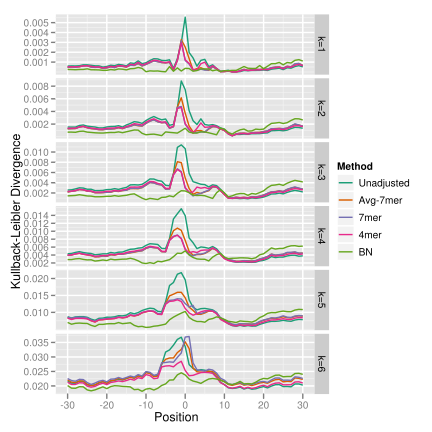
\includegraphics[width=0.5\textwidth]{fig/cao-kl.pdf}
\end{center}

We see that our method is effective at reducing the bias in this ChIP-Seq data.



\section{Bias in Amplification-Free Sequencing}

To evaluate the extent to which the observed bias is caused by PCR amplification
in the library preparation stage, we analyzed data from the FRT-Seq protocol
developed by Mamanova, et. al. \cite{Mamanova2010}. FRT-Seq avoids the
amplification step during library preparation with reverse transcription
occuring on the flowcell surface. We obtained data generated by Mamanova, et.
al., from the European Nucleotide Archive with accession code ERR007689, and
mapped them to the hg19 assembly of the human genome with Bowtie
\cite{Langmead2009}. The nucleotide frequencies and divergence are plotted
below.

\begin{center}
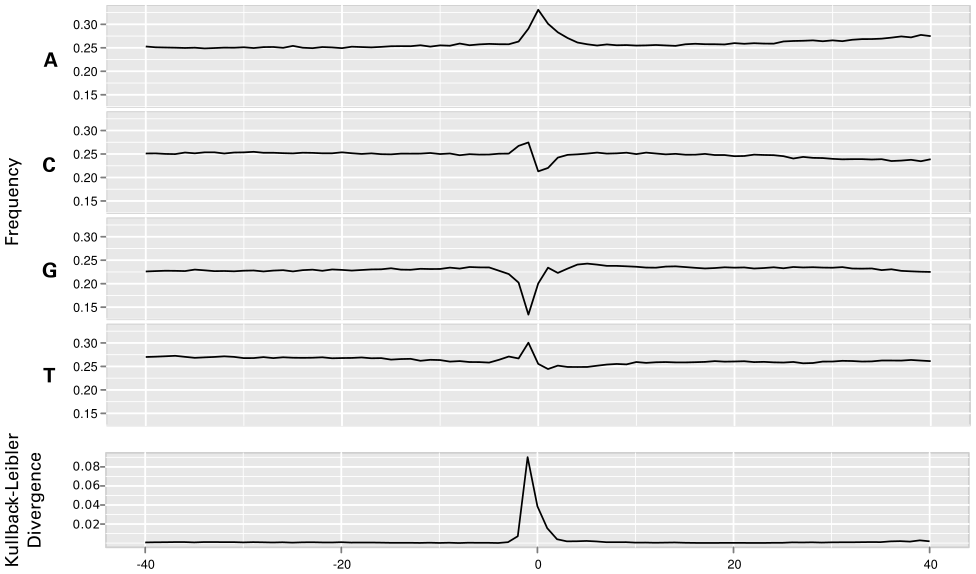
\includegraphics[width=0.6\textwidth]{fig/frt-all.pdf}
\end{center}

It is clear from this analysis that the FRT-Seq method, as implemented to
generate this data, is not without bias, yet there is significant divergence at
only a small number of positions surrounding the read start. When our method is
trained on this data we obtain the suitably sparse model pictured below.

\begin{center}
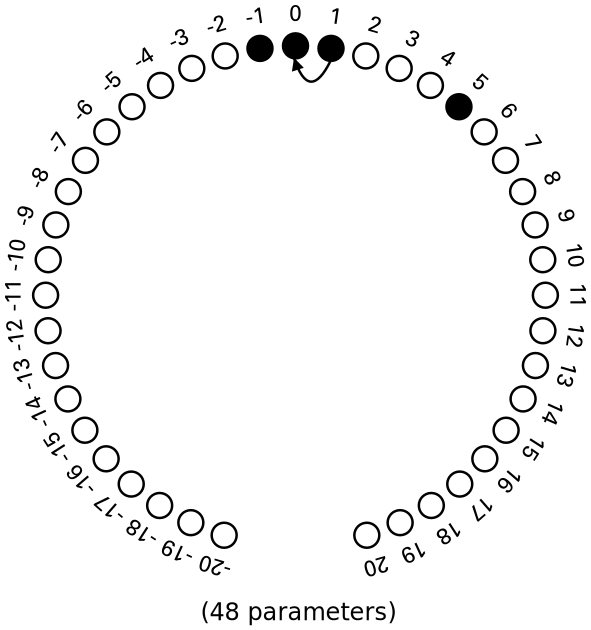
\includegraphics[width=0.4\textwidth]{fig/frt-graph.pdf}
\end{center}



\section{Variability Between Replicates}

Measuring differential expression or isoform switching is a primary application of
RNA-Seq. If the bias were inconsistent between replicates, it would call into
question the accuracy of such tests. In our experiments, we have observed the
bias to be mostly, but not entirely consistent between replicates. Below, we
plot the frequencies from the four runs in the Trapnell data set.

\begin{center}
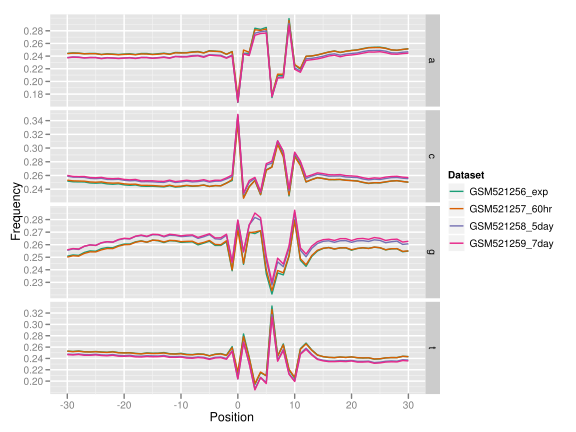
\includegraphics[width=0.5\textwidth]{fig/replicates.pdf}
\end{center}

Though we do not know if the variability is always minor, assuming this is so,
there remains the risk that the sequence bias would greatly effect the depth to
which a locus is sequenced, and thus the statistical significance of
differential expression tests. This would bias the discovery of differentially
expressed genes, but not the test itself.



\section{Comparison to qRT-PCR}

We used sequencing data previously published by Au, et al, \cite{Au2010} to
evalute the effect bias correction has on correlation to measurements made by
TaqMan RT-PCR, made available by the Microarray Quality Control project
\cite{Shi2006}. The RNA-Seq data shows a pattern of bias similar to that seen in
other samples sequenced on an Illumina platform, as plotted below.

\centerline{\includegraphics[width=0.6\textwidth]{fig/au-freqs.pdf}}

To evaluate the efficacy of each of the bias correction methods considered, 

We counted reads overlapping each gene, defining the gene by the union of every
transcript annotated in release 62 of the Ensembl gene annotations, excluding
UTRs, and 100 additional bases from both ends of the gene. Counts were then
normalized (divided) by the adjusted length of these genes.  We then remove any
genes with reads fewer than 10 reads, or without a unique TaqMan probe, leaving
592 genes.

Each bias correction method was trained using a procedure identical to the one
described in the results section. After adjusting read counts according to the
predicted sequence bias, we compute the Pearson correlation between log read counts
and log TaqMan expression values, which are averaged across three replicates. The
expression values 

These correlations are listed below.

\begin{center}
\begin{tabular}{ll}
\textbf{Method} & \textbf{Correlation} \\ \hline
Unadjusted &  0.6665 \\
7mer &  0.6677 \\
GLM & 0.6854 \\
MART & 0.6921 \\
BN & 0.7016
\end{tabular}
\end{center}

These results are consistent with with the KL-divergence and Poisson regression
analysis presented in Section 3. We see only very small gains with the
brute-force 7mer method. The GLM and MART models show much better performance,
and our Baysian network (BN) method shows moderate increase correlation over these.


\bibliographystyle{plain}
\bibliography{seqbias-paper}

\end{document}




